\chapter{NMR Lebih Dalam: Pulsa, Relaksasi, dan 2D}\label{ch:b3:advanced-nmr}

Pemindai MRI di rumah sakit dan spektrometer NMR di sebuah jurusan kimia
bekerja dengan prinsip yang sama. Keduanya menempatkan inti-inti hidrogen
dalam medan magnet yang kuat, memiringkan magnetisasinya dengan pulsa
gelombang radio yang singkat, lalu mendengarkan sinyal lemah yang
diinduksinya ketika magnetisasi itu berpresesi dan berelaksasi. Pemindai
mengubah sinyal itu menjadi citra jaringan lunak; spektrometer mengubahnya
menjadi daftar pergeseran kimia dan kopling, dan, dengan beberapa pulsa
berturut-turut, menjadi peta dua dimensi yang memperlihatkan atom mana yang
terikat pada atom mana. Bab ini menjelaskan apa yang dilakukan pulsa-pulsa
itu, mengapa sinyalnya memudar, dan bagaimana \omterm{def:b3:advanced-nmr:two-d}{spektrum dua dimensi} dibaca
--- metode yang kini dipakai untuk memecahkan sebagian besar struktur
organik baru.

\begin{recall}
Jilid Tahun 1 menafsirkan spektrum NMR ${}^1$H: pergeseran kimia, perisaian,
proton ekuivalen, integrasi, kopling spin--spin, tetapan kopling, dan
multiplet. Jilid Tahun 2 menambahkan NMR ${}^{13}$C dengan dekopling pita lebar
dan DEPT, yang deret pulsanya diterima begitu saja; pulsa-pulsa itu dijelaskan
di sini. \Cref{ch:b3:many-electron-atoms} memperlakukan spin sebagai momentum
sudut. Dari fisika: momen magnetik dalam medan mempunyai energi
$-\boldsymbol\mu\cdot\mathbf B$, dan populasi tingkat-tingkat energi mengikuti
faktor Boltzmann $\eu^{-\Delta E/kT}$, yang dikembangkan dalam
\cref{ch:b3:partition-functions}.
\end{recall}

\begin{omfigure}
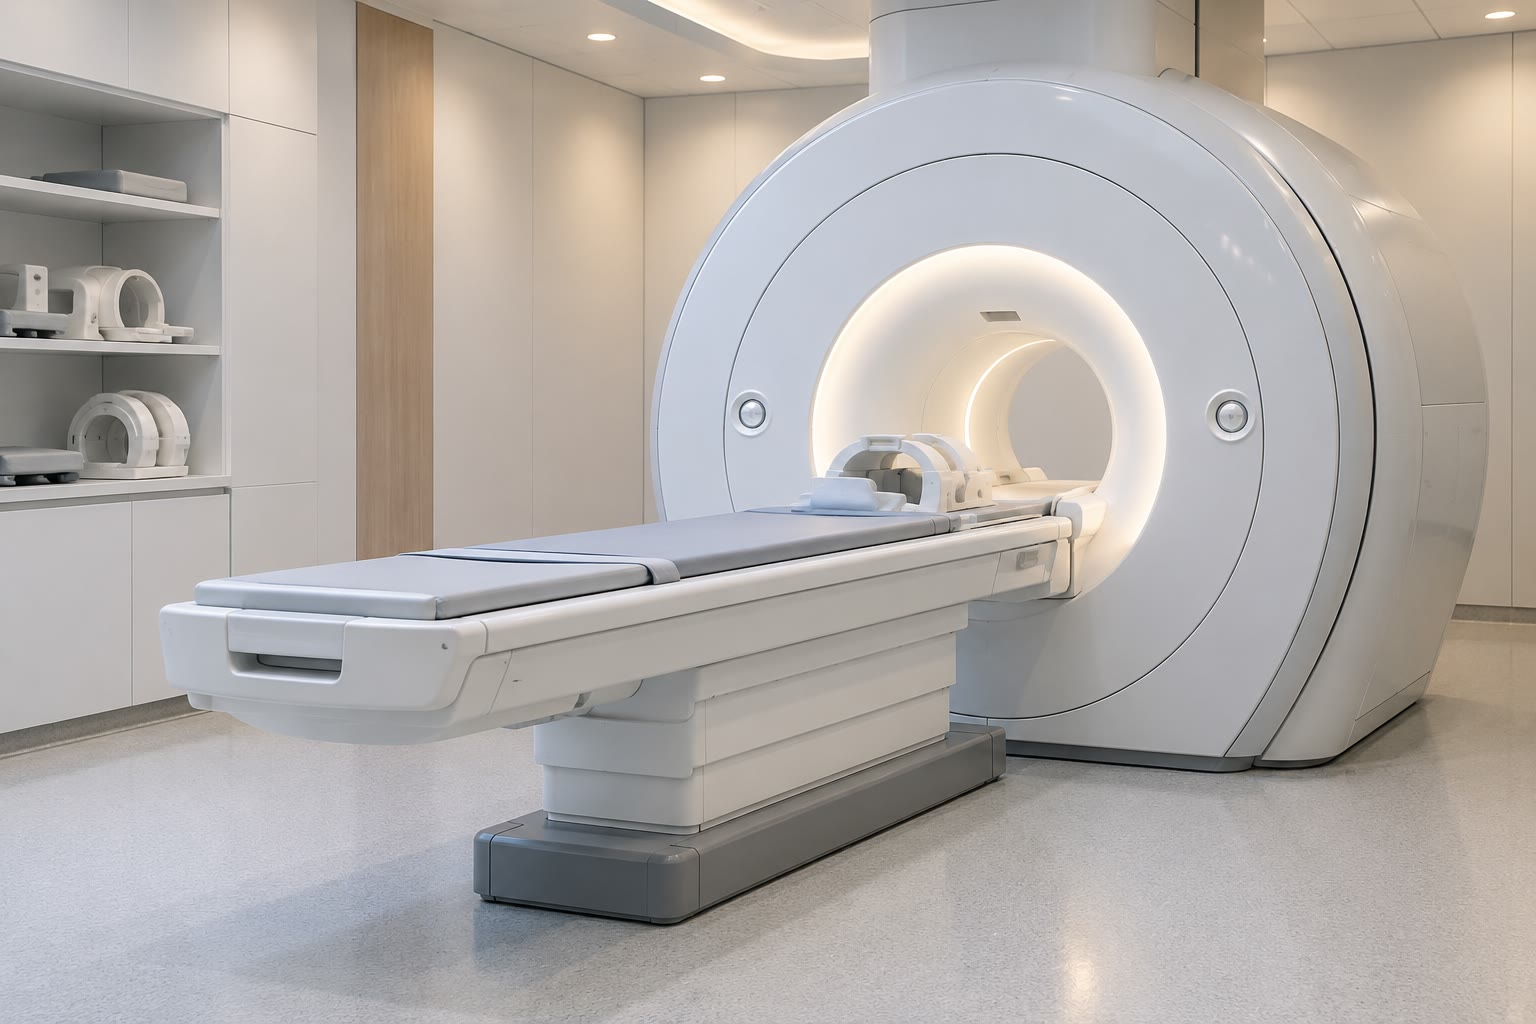
\includegraphics[width=0.52\linewidth]{images/book4/ai/b3-08-mri.jpg}\hspace{0.8em}%
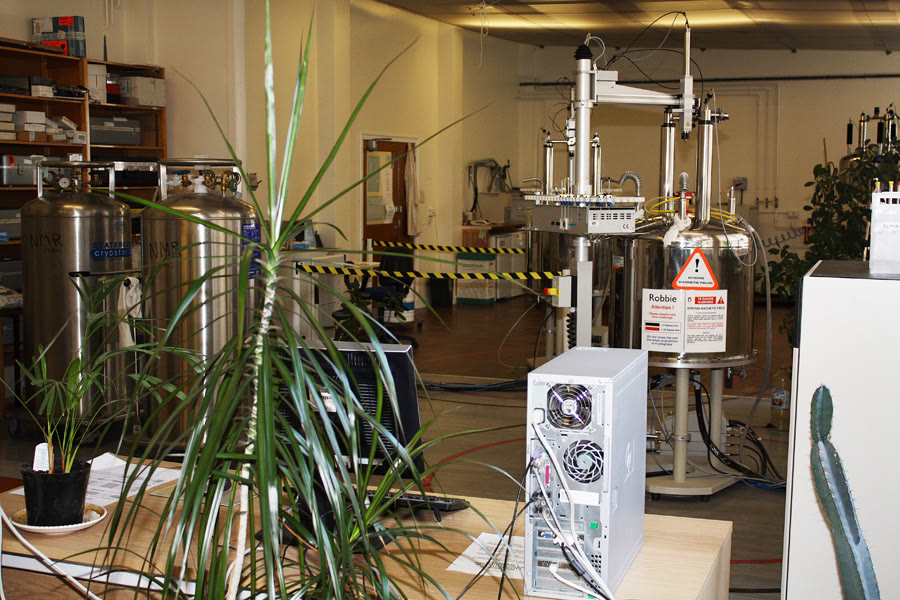
\includegraphics[width=0.4\linewidth]{images/book4/nmr-lab.jpg}

{\small Kiri: pemindai MRI rumah sakit. Kanan: laboratorium NMR; setiap
magnet superkonduktor berdiri di dalam kriostatnya, yang diisi ulang dengan
helium cair dan nitrogen cair dari dewar di sebelah kiri. Foto Shandchem,
CC\ BY\ 2.0.}
\end{omfigure}

\section{Spin inti dalam medan magnet}

\begin{definition}[Bilangan kuantum spin inti, rasio giromagnetik]\label{def:b3:advanced-nmr:nuclear-spin}
Sebuah inti mempunyai momentum sudut spin dengan bilangan kuantum $I$, yang
disebut \emph{bilangan kuantum spin inti}\index{bilangan kuantum spin inti}
($I = 0$ untuk \ce{^{12}C}, \ce{^{16}O}; $\frac12$ untuk \ce{^1H}, \ce{^{13}C},
\ce{^{15}N}, \ce{^{19}F}, \ce{^{31}P}; 1 untuk \ce{^2H}, \ce{^{14}N}), dan momen
magnetik $\boldsymbol\mu = \gamma\hat{\mathbf
I}$ yang sebanding dengannya; $\gamma$ disebut \emph{rasio
giromagnetik}\index{rasio giromagnetik}. Sepanjang medan $B_0$ (sumbu $z$),
$\hat I_z$ mengambil nilai-nilai $m_I\hbar$, $m_I = -I, \dots, I$.
\end{definition}

\begin{proposition}[Tingkat-tingkat Zeeman]\label{prop:b3:advanced-nmr:zeeman}
Dalam medan $B_0$, tingkat-tingkat energinya adalah $E_m = -m_I\gamma\hbar B_0$;
transisi $\Delta m_I = \pm1$ menyerap pada frekuensi
\[
\nu_0 = \frac{\gamma B_0}{2\pi}.
\]
\end{proposition}

\begin{proof}
$E = -\boldsymbol\mu\cdot\mathbf B = -\gamma B_0\hat I_z$, dengan \omterm{def:b3:quantum-model-systems:operator}{nilai eigen}
$-\gamma B_0m_I\hbar$. Tingkat-tingkat yang bersebelahan berselisih
$\gamma\hbar B_0 = h\nu_0$.
\end{proof}

\begin{definition}[Frekuensi Larmor]\label{def:b3:advanced-nmr:larmor}
$\nu_0 = \gamma B_0/2\pi$ disebut \emph{frekuensi Larmor}\index{frekuensi Larmor}
inti itu: frekuensi resonansinya, dan juga frekuensi presesi momen
magnetiknya terhadap medan.
\end{definition}

\begin{example}[Inti-inti yang umum]\label{ex:b3:advanced-nmr:nuclei}
% ledger: const:gammaP, nuc:C13.mu, nuc:F19.mu, nuc:P31.mu, nuc:N15.mu, const:muN
Untuk inti berspin $\frac12$ dengan momen $\mu$, $\gamma/2\pi = \mu/(Ih) = 2\mu/h$.
Dengan momen-momen terukur: \ce{^1H} \qty{42.58}{MHz/T}, \ce{^{19}F}
\qty{40.08}{MHz/T}, \ce{^{31}P} \qty{17.25}{MHz/T}, \ce{^{13}C}
\qty{10.71}{MHz/T}, \ce{^{15}N} \qty{-4.32}{MHz/T}. ``Spektrometer
\qty{400}{MHz}'' mempunyai $B_0 = \qty{9.4}{T}$: proton-protonnya beresonansi
pada \qty{400.2}{MHz}, karbon-karbonnya pada \qty{100.7}{MHz}.
\end{example}

\begin{proposition}[Selisih populasi yang sangat kecil]\label{prop:b3:advanced-nmr:populations}
Untuk spin $\frac12$ pada suhu $T$, kelebihan inti pada tingkat bawah adalah
\[
\frac{N_\alpha - N_\beta}{N} \approx \frac{\gamma\hbar B_0}{2kT}.
\]
\end{proposition}

\begin{proof}
$N_\beta/N_\alpha = \eu^{-\Delta E/kT} \approx 1 - \Delta E/kT$ karena
$\Delta E \ll kT$; jadi $(N_\alpha - N_\beta)/(N_\alpha + N_\beta) \approx \Delta E/2kT$,
dengan $\Delta E = \gamma\hbar B_0$.
\end{proof}

Untuk proton pada \qty{9.4}{T} dan \qty{300}{K} kelebihannya \num{3.2e-5}: hanya
tiga inti dari seratus ribu yang menyumbang. Karena kelebihan itu dan
tegangan yang diinduksi dalam kumparan sama-sama tumbuh bersama $\gamma$ dan
$B_0$, sinyalnya tumbuh kira-kira sebanding dengan $\gamma^3B_0^2$: itulah alasan
dibuatnya magnet yang makin kuat, dan alasan rendahnya kepekaan inti dengan
$\gamma$ kecil dan kelimpahan alami rendah seperti \ce{^{13}C}.

\section{Pulsa dan peluruhan induksi bebas}

\begin{definition}[Magnetisasi neto, kerangka berputar]\label{def:b3:advanced-nmr:magnetisation}
Yang disebut \emph{magnetisasi neto}\index{magnetisasi neto} $\mathbf M$ sebuah
sampel adalah jumlah momen-momen magnetik intinya per satuan volume; pada
kesetimbangan, magnetisasi itu sebesar $M_0$ sepanjang $\mathbf B_0$. Yang
disebut \emph{kerangka berputar}\index{kerangka berputar} adalah sistem sumbu
$x'$, $y'$, $z$ yang berputar terhadap $z$ dengan frekuensi gelombang radio
yang diberikan; di dalamnya presesi pada $\nu_0$ terlihat melambat menjadi
selisih $\nu_0 -
\nu_{\mathrm{rf}}$.
\end{definition}

\begin{proposition}[Presesi]\label{prop:b3:advanced-nmr:precession}
Magnetisasi dalam sebuah medan mematuhi $\dd\mathbf M/\dd t = \gamma\,\mathbf M\times\mathbf B$;
dalam medan statis $B_0\mathbf e_z$, komponen transversalnya berputar terhadap
$z$ dengan frekuensi sudut $\omega_0 = \gamma B_0$, sedangkan $M_z$ tetap.
\end{proposition}

\begin{proof}[Bukti parsial]
Persamaan itu adalah persamaan torsi klasik untuk momen magnetik yang membawa
momentum sudut, yang diterima dari fisika. Dengan $\mathbf B = B_0\mathbf e_z$:
$\dot M_x = \gamma
B_0M_y$, $\dot M_y = -\gamma B_0M_x$, $\dot M_z = 0$, yang solusinya adalah
$M_x + \iu M_y \propto
\eu^{-\iu\gamma B_0t}$: rotasi pada $\omega_0$ (searah jarum jam dilihat dari $+z$
untuk $\gamma > 0$).
\end{proof}

\begin{definition}[Pulsa frekuensi radio, sudut balik]\label{def:b3:advanced-nmr:pulse}
Yang disebut \emph{pulsa frekuensi radio}\index{pulsa frekuensi radio} adalah
semburan singkat gelombang radio pada $\nu_{\mathrm{rf}} \approx \nu_0$, yang medan
magnetiknya $B_1$, tetap sepanjang $x'$ dalam \omterm{def:b3:advanced-nmr:magnetisation}{kerangka berputar}, memutar
$\mathbf M$ terhadap $x'$. Sudut putaran itu disebut \emph{sudut
balik}\index{sudut balik} $\theta = \gamma B_1t_p$ untuk pulsa berdurasi $t_p$:
pulsa $90^\circ$ membawa $\mathbf M$ ke bidang $x'y'$, pulsa $180^\circ$
membaliknya.
\end{definition}

\begin{omfigure}
\tdplotsetmaincoords{70}{120}
\begin{tikzpicture}[tdplot_main_coords, font=\small, >=Stealth]
  \begin{scope}
    \draw[->, gray] (0,0,0) -- (1.8,0,0) node[anchor=north east] {$x'$};
    \draw[->, gray] (0,0,0) -- (0,1.8,0) node[anchor=north west] {$y'$};
    \draw[->, gray] (0,0,0) -- (0,0,1.8) node[anchor=south] {$z$, $\mathbf B_0$};
    \draw[->, omThm, very thick] (0,0,0) -- (0,0,1.4) node[anchor=west] {$\mathbf M$};
    \node[anchor=north] at (0,0,-0.9) {kesetimbangan};
  \end{scope}
  \begin{scope}[shift={(0,4.6,0)}]
    \draw[->, gray] (0,0,0) -- (1.8,0,0) node[anchor=north east] {$x'$};
    \draw[->, gray] (0,0,0) -- (0,1.8,0) node[anchor=north west] {$y'$};
    \draw[->, gray] (0,0,0) -- (0,0,1.8) node[anchor=south] {$z$};
    \draw[->, omDef, thick] (0,0,0) -- (1.2,0,0) node[anchor=south east, xshift=-2pt] {$\mathbf B_1$};
    \draw[->, omThm, very thick] (0,0,0) -- (0,1.4,0) node[anchor=south west] {$\mathbf M$};
    \node[anchor=north] at (0,0,-0.9) {setelah pulsa $90^\circ_{x'}$};
  \end{scope}
  \begin{scope}[shift={(0,9.2,0)}]
    \draw[->, gray] (0,0,0) -- (1.8,0,0) node[anchor=north east] {$x'$};
    \draw[->, gray] (0,0,0) -- (0,1.8,0) node[anchor=north west] {$y'$};
    \draw[->, gray] (0,0,0) -- (0,0,1.8) node[anchor=south] {$z$};
    \draw[->, omThm, very thick] (0,0,0) -- (0,0,-1.4) node[anchor=west] {$\mathbf M$};
    \node[anchor=north] at (0,0,-1.6) {setelah pulsa $180^\circ_{x'}$};
  \end{scope}
\end{tikzpicture}

{\small Magnetisasi dalam \omterm{def:b3:advanced-nmr:magnetisation}{kerangka berputar}. Pulsa $90^\circ$ terhadap $x'$
memutar $\mathbf M$ dari $z$ ke $y'$ (dengan $\gamma > 0$ rotasinya mengikuti
aturan tangan kiri terhadap $\mathbf B_1$, sesuai konvensi yang lazim); pulsa
$180^\circ$ membaliknya.}
\end{omfigure}

\begin{definition}[Peluruhan induksi bebas]\label{def:b3:advanced-nmr:fid}
Setelah pulsa $90^\circ$, magnetisasi transversal berpresesi pada \omterm{def:b3:advanced-nmr:larmor}{frekuensi
Larmor} dan menginduksi tegangan bolak-balik dalam kumparan di sekitar sampel,
yang meredup ketika magnetisasi itu berelaksasi: inilah \emph{peluruhan
induksi bebas}\index{peluruhan induksi bebas} (FID).
\end{definition}

\begin{theorem}[Dari FID ke spektrum]\label{thm:b3:advanced-nmr:lorentzian}
Transformasi Fourier osilasi yang meluruh $\eu^{-t/T_2}\cos(2\pi\nu t)$ ($t \ge 0$)
adalah, di dekat $\nu$, garis Lorentz dengan lebar penuh pada setengah
maksimum $1/(\pi T_2)$.
\end{theorem}

\begin{proof}
Tuliskan sinyalnya sebagai $\eu^{-t/T_2}\eu^{2\pi\iu\nu t}$ lalu integralkan:
$\int_0^\infty\eu^{-t/T_2}\eu^{2\pi\iu(\nu - f)t}\dd t = \frac{1}{1/T_2 - 2\pi\iu(\nu - f)}$, yang
bagian realnya adalah $\frac{T_2}{1 + 4\pi^2T_2^2(f - \nu)^2}$. Bagian real itu
maksimum pada $f = \nu$ dan turun menjadi setengahnya ketika
$2\pi T_2|f - \nu| = 1$, yaitu pada $f - \nu = \pm1/(2\pi T_2)$: lebar penuh
$1/(\pi T_2)$.
\end{proof}

\begin{omfigure}
\begin{tikzpicture}
\begin{axis}[name=fid, width=0.5\linewidth, height=4.6cm, xmin=0, xmax=0.4,
  ymin=-2.1, ymax=2.1, axis lines=left, xlabel={$t$ / s}, ylabel={sinyal},
  ytick=\empty, scaled x ticks=false, xticklabel style={/pgf/number format/fixed},
  tick label style={font=\small}, label style={font=\small}, title={\small FID}]
\addplot[omDef] table[x=t, y=s] {figdata/out/bachelor-3-nmr-fid.dat};
\addplot[gray, dashed, domain=0:0.4, samples=60] {2*exp(-x/0.1)};
\end{axis}
\begin{axis}[at={(fid.east)}, anchor=west, xshift=1.2cm, width=0.45\linewidth,
  height=4.6cm, xmin=0, xmax=350, ymin=-0.1, ymax=1.1, axis x line=bottom,
  axis y line=none, xlabel={frekuensi relatif / Hz}, tick label style={font=\small},
  label style={font=\small}, title={\small spektrum (transformasi Fourier)}]
\addplot[omThm, thick] table[x=f, y=I] {figdata/out/bachelor-3-nmr-fid-spectrum.dat};
\end{axis}
\end{tikzpicture}

{\small Kiri: FID dua garis (frekuensi relatif 100 dan \qty{250}{Hz},
$T_2 = \qty{0.10}{s}$), yang berdenyut karena kedua frekuensi berinterferensi
di dalam selubung eksponensial (garis putus-putus). Kanan: transformasi
Fouriernya, dua garis Lorentz selebar \qty{3.2}{Hz}.}
\end{omfigure}

\begin{proposition}[Perataan sinyal]\label{prop:b3:advanced-nmr:averaging}
Menjumlahkan $N$ FID mengalikan sinyalnya dengan $N$ dan derau acaknya dengan
$\sqrt N$: rasio sinyal terhadap derau tumbuh sebanding dengan $\sqrt N$.
\end{proposition}

\begin{proof}
Sinyalnya bertambah secara koheren. Derau akuisisi-akuisisi yang saling
bebas masing-masing mempunyai rata-rata nol dan variansi $\sigma^2$; variansi
jumlah $N$ suku yang saling bebas adalah $N\sigma^2$ (hukum perambatan dalam jilid
Tahun 2), sehingga simpangan bakunya $\sqrt N\sigma$.
\end{proof}

DEPT, yang memilah sinyal ${}^{13}$C menurut banyaknya hidrogen yang terikat,
mengenakan sederet pulsa pada proton dan karbon yang dipisahkan oleh jeda
$1/2J$: magnetisasi proton yang besar dipindahkan ke karbon melalui kopling
satu ikatan, yang mengalikan sinyal karbon dengan sekitar
$\gamma_H/\gamma_C \approx 4$, dan sudut pulsa proton yang terakhir memberi bobot
berbeda pada CH, \ce{CH2} dan \ce{CH3}. Gagasan yang sama --- memindahkan
magnetisasi antarinti melalui kopling-koplingnya --- mendasari
eksperimen-eksperimen dua dimensi di bawah ini.

\section{Relaksasi}

\begin{definition}[Waktu relaksasi longitudinal dan transversal]\label{def:b3:advanced-nmr:relaxation}
Kembalinya $M_z$ ke $M_0$ setelah sebuah gangguan berlangsung secara
eksponensial, dengan \emph{waktu relaksasi
longitudinal}\index{waktu relaksasi longitudinal} $T_1$ (relaksasi spin--kisi: energi diserahkan ke lingkungan).
Peluruhan magnetisasi transversal ke nol berlangsung secara eksponensial
dengan \emph{waktu relaksasi transversal}\index{waktu relaksasi transversal}
$T_2 \le T_1$ (relaksasi spin--spin: hilangnya koherensi fase antarspin).
\end{definition}

\begin{proposition}[Pemulihan inversi]\label{prop:b3:advanced-nmr:inversion-recovery}
Setelah pulsa $180^\circ$, $M_z(t) = M_0(1 - 2\eu^{-t/T_1})$; magnetisasi itu
melewati nol pada $t_{\mathrm{null}} = T_1\ln2$.
\end{proposition}

\begin{proof}
Persamaan relaksasi $\dd M_z/\dd t = (M_0 - M_z)/T_1$ dengan $M_z(0) = -M_0$
mempunyai solusi $M_0 - 2M_0\eu^{-t/T_1}$, yang lenyap ketika
$\eu^{-t/T_1} = \frac12$.
\end{proof}

\begin{method}[Mengukur $T_1$ dan menetapkan jeda ulang yang kuantitatif]\label{met:b3:advanced-nmr:t1}
\begin{enumerate}
  \item Jalankan deret $180^\circ$--$\tau$--$90^\circ$--akuisisi untuk sederet jeda
        $\tau$, dengan menunggu sedikitnya $5T_1$ antarpindaian.
  \item Cocokkan setiap sinyal dengan $M_0(1 - 2\eu^{-\tau/T_1})$, atau bacalah
        titik nolnya: $T_1 =
        t_{\mathrm{null}}/\ln2$.
  \item Untuk integrasi kuantitatif dengan pulsa $90^\circ$, tunggulah
        sedikitnya $5T_1$ inti yang paling lambat antarpindaian: dengan begitu
        bagian magnetisasi yang hilang $\eu^{-5} < 1\,\%$.
\end{enumerate}
\end{method}

\begin{omfigure}
\begin{tikzpicture}
\begin{axis}[width=0.62\linewidth, height=5cm, xmin=0, xmax=10, ymin=-1.1, ymax=1.15,
  axis lines=left, xlabel={$t$ / s}, ylabel={$M/M_0$}, legend cell align=left,
  legend style={font=\small, draw=none, at={(0.97,0.05)}, anchor=south east},
  tick label style={font=\small}, label style={font=\small}]
\addplot[omDef, thick] table[x=t, y=mz] {figdata/out/bachelor-3-nmr-relaxation.dat};
\addlegendentry{$M_z$ setelah $180^\circ$ ($T_1 = \qty{2.0}{s}$)}
\addplot[omThm, thick, dashed] table[x=t, y=mxy] {figdata/out/bachelor-3-nmr-relaxation.dat};
\addlegendentry{$M_{xy}$ setelah $90^\circ$ ($T_2 = \qty{0.5}{s}$)}
\addplot[gray, dotted, domain=0:10] {0};
\addplot[only marks, mark=*, mark size=1.5pt, black] coordinates {(1.386,0)};
\node[font=\small, anchor=north west] at (axis cs:1.5,-0.04) {$T_1\ln2$};
\end{axis}
\end{tikzpicture}

{\small Relaksasi (nilai-nilai model). Magnetisasi longitudinal yang
terbalik pulih melewati nol pada $T_1\ln2$; magnetisasi transversal meluruh
lebih cepat, dengan $T_2$.}
\end{omfigure}

\begin{definition}[Gema spin]\label{def:b3:advanced-nmr:echo}
Dalam deret $90^\circ$--$\tau$--$180^\circ$--$\tau$, spin-spin yang fasenya saling
menjauh karena ketakhomogenan medan difokuskan kembali pada waktu $2\tau$,
sehingga menghasilkan sebuah \emph{gema spin}\index{gema spin}; amplitudonya
meluruh dengan $T_2$ yang sebenarnya, bebas dari ketakhomogenan magnet.
\end{definition}

\begin{definition}[Efek Overhauser inti]\label{def:b3:advanced-nmr:noe}
Menjenuhkan atau mengganggu sebuah spin mengubah, melalui relaksasi dipolar,
intensitas sinyal spin lain yang dekat dalam ruang: inilah \emph{efek
Overhauser inti}\index{efek Overhauser inti} (NOE). Laju pertumbuhannya
sebanding dengan $r^{-6}$, sehingga efek itu hanya terlihat antara inti-inti
yang berjarak kurang dari sekitar \qty{0.5}{nm}, baik terikat maupun tidak.
\end{definition}

\section{NMR dua dimensi}

\begin{definition}[Spektrum dua dimensi, puncak silang, puncak diagonal]\label{def:b3:advanced-nmr:two-d}
Yang disebut \emph{spektrum dua dimensi}\index{spektrum dua dimensi} adalah
spektrum yang direkam dengan mengulang sebuah deret pulsa dengan jeda $t_1$
yang dinaikkan bertahap sebelum waktu akuisisi $t_2$; transformasi Fourier
ganda memberikan peta intensitas terhadap dua frekuensi. Sebuah \emph{puncak
silang}\index{puncak silang} pada $(\delta_1,
\delta_2)$ menunjukkan bahwa inti-inti pada $\delta_1$ dan $\delta_2$ terhubung
(melalui kopling atau melalui kedekatan); sebuah \emph{puncak
diagonal}\index{puncak diagonal} pada $(\delta, \delta)$ milik satu inti saja.
\end{definition}

\begin{definition}[COSY, HSQC, HMBC, NOESY]\label{def:b3:advanced-nmr:experiments}
\emph{COSY}\index{COSY} (spektroskopi korelasi) mengorelasikan proton-proton
yang saling berkopling, biasanya melalui tiga ikatan (H--C--C--H).
\emph{HSQC}\index{HSQC} (koherensi kuantum tunggal heteronuklir) mengorelasikan
setiap karbon dengan proton-proton yang terikat langsung padanya.
\emph{HMBC}\index{HMBC} (korelasi ikatan jamak heteronuklir) mengorelasikan
karbon-karbon dengan proton-proton yang berjarak dua atau tiga ikatan,
melintasi karbon kuaterner dan heteroatom. \emph{NOESY}\index{NOESY}
mengorelasikan proton-proton yang berdekatan dalam ruang melalui \omterm{def:b3:advanced-nmr:noe}{efek
Overhauser inti}.
\end{definition}

\begin{omfigure}
\begin{tikzpicture}[font=\small]
  \foreach \y/\name in {3.2/{satu pulsa}, 2.0/{pemulihan inversi}, 0.8/{gema spin}, -0.4/{COSY}}{
    \draw (0,\y) -- (9.3,\y); \node[anchor=east] at (-0.1,\y+0.25) {\name};}
  % one pulse
  \fill[black] (0.4,3.2) rectangle (0.6,3.75);
  \draw[omDef, domain=0:3.5, samples=120] plot (0.7+\x, {3.2+0.4*exp(-\x/1.2)*sin(\x*500)});
  % inversion recovery
  \fill[black] (0.4,2.0) rectangle (0.8,2.55); \node[font=\scriptsize] at (0.6,2.7) {180};
  \draw[<->] (0.85,1.85) -- (2.4,1.85) node[midway, below, font=\scriptsize] {$\tau$};
  \fill[black] (2.45,2.0) rectangle (2.65,2.55); \node[font=\scriptsize] at (2.55,2.7) {90};
  \draw[omDef, domain=0:3.0, samples=120] plot (2.75+\x, {2.0+0.4*exp(-\x/1.0)*sin(\x*500)});
  % spin echo
  \fill[black] (0.4,0.8) rectangle (0.6,1.35); \node[font=\scriptsize] at (0.5,1.5) {90};
  \draw[<->] (0.65,0.65) -- (2.4,0.65) node[midway, below, font=\scriptsize] {$\tau$};
  \fill[black] (2.45,0.8) rectangle (2.85,1.35); \node[font=\scriptsize] at (2.65,1.5) {180};
  \draw[<->] (2.9,0.65) -- (4.65,0.65) node[midway, below, font=\scriptsize] {$\tau$};
  \draw[omDef, domain=-1.2:2.5, samples=150] plot (4.65+\x, {0.8+0.35*exp(-abs(\x)/0.35)*cos(\x*700)});
  % COSY
  \fill[black] (0.4,-0.4) rectangle (0.6,0.15); \node[font=\scriptsize] at (0.5,0.3) {90};
  \draw[<->] (0.65,-0.55) -- (2.4,-0.55) node[midway, below, font=\scriptsize] {$t_1$ (dinaikkan bertahap)};
  \fill[black] (2.45,-0.4) rectangle (2.65,0.15); \node[font=\scriptsize] at (2.55,0.3) {90};
  \draw[omDef, domain=0:3.0, samples=120] plot (2.75+\x, {-0.4+0.4*exp(-\x/1.0)*sin(\x*500)});
  \node[font=\scriptsize, anchor=west] at (5.9,-0.2) {akuisisi ($t_2$)};
\end{tikzpicture}

{\small Deret-deret pulsa (waktu ke kanan; kotak penuh: pulsa, dilabeli dengan
\omterm{def:b3:advanced-nmr:pulse}{sudut baliknya} dalam derajat; biru: sinyal yang direkam). \omterm{def:b3:advanced-nmr:echo}{Gema spin} mencapai
puncaknya pada $2\tau$ setelah pulsa pertama.}
\end{omfigure}

\begin{method}[Memecahkan struktur dengan spektrum dua dimensi]\label{met:b3:advanced-nmr:solve-2d}
\begin{enumerate}
  \item Dari rumus molekul, integral ${}^1$H, dan spektrum ${}^{13}$C/DEPT,
        daftarlah karbon CH, \ce{CH2}, \ce{CH3}, dan karbon kuaterner.
  \item \omterm{def:b3:advanced-nmr:experiments}{HSQC}: pasangkan setiap sinyal proton dengan karbonnya.
  \item \omterm{def:b3:advanced-nmr:experiments}{COSY}: gabungkan karbon-karbon yang berproton menjadi sistem-sistem
        spin (rantai tetangga).
  \item \omterm{def:b3:advanced-nmr:experiments}{HMBC}: hubungkan sistem-sistem spin melintasi karbon kuaterner,
        karbonil, dan heteroatom, tempat \omterm{def:b3:advanced-nmr:experiments}{COSY} tidak memberi sinyal.
  \item \omterm{def:b3:advanced-nmr:experiments}{NOESY}: tetapkan konfigurasi relatif dan konformasi dari kontak-kontak
        melalui ruang.
  \item Periksalah setiap sinyal terhadap struktur yang diusulkan.
\end{enumerate}
\end{method}

\begin{omfigure}
\begin{tikzpicture}
\begin{axis}[name=cosy, width=0.47\linewidth, height=0.47\linewidth, x dir=reverse,
  y dir=reverse, xmin=0.5, xmax=4.6, ymin=0.5, ymax=4.6, axis lines=box,
  xlabel={$\delta_{\mathrm H}$ / ppm}, ylabel={$\delta_{\mathrm H}$ / ppm},
  tick label style={font=\small}, label style={font=\small}, title={\small COSY}]
\addplot[gray, dotted, domain=0.5:4.6] {x};
\addplot[only marks, mark=*, mark size=2.2pt, black] table[x=h1, y=h2] {figdata/out/bachelor-3-nmr-2d-cosy-diag.dat};
\addplot[only marks, mark=*, mark size=2.2pt, omThm] table[x=h1, y=h2] {figdata/out/bachelor-3-nmr-2d-cosy-cross.dat};
\end{axis}
\begin{axis}[at={(cosy.east)}, anchor=west, xshift=1.3cm, width=0.47\linewidth,
  height=0.47\linewidth, x dir=reverse, y dir=reverse, xmin=0.5, xmax=4.6,
  ymin=0, ymax=185, axis lines=box, xlabel={$\delta_{\mathrm H}$ / ppm},
  ylabel={$\delta_{\mathrm C}$ / ppm}, tick label style={font=\small},
  label style={font=\small}, title={\small HSQC (biru) dan HMBC (merah)}]
\addplot[only marks, mark=square*, mark size=2.2pt, omDef] table[x=h, y=c] {figdata/out/bachelor-3-nmr-2d-hsqc.dat};
\addplot[only marks, mark=o, mark size=2.6pt, omThm, thick] table[x=h, y=c] {figdata/out/bachelor-3-nmr-2d-hmbc.dat};
\end{axis}
\end{tikzpicture}

{\small \omterm{def:b3:advanced-nmr:two-d}{Spektrum dua dimensi} etil butanoat, \ce{CH3CH2CH2COOCH2CH3}, yang
digambar pada pergeseran-pergeseran terukurnya. \omterm{def:b3:advanced-nmr:experiments}{COSY}: hitam, \omterm{def:b3:advanced-nmr:two-d}{puncak diagonal};
merah, \omterm{def:b3:advanced-nmr:two-d}{puncak silang} antara proton-proton pada karbon-karbon yang bertetangga
--- dua sistem spin, etil dan propil, tanpa \omterm{def:b3:advanced-nmr:two-d}{puncak silang} yang melintasi
oksigen ester. Kanan: puncak \omterm{def:b3:advanced-nmr:experiments}{HSQC} (persegi) memasangkan setiap proton dengan
karbonnya; puncak \omterm{def:b3:advanced-nmr:experiments}{HMBC} (lingkaran) memperlihatkan proton OCH$_2$
(\qty{4.13}{ppm}) dan proton CH$_2$C=O (\qty{2.28}{ppm}) yang sama-sama mencapai
karbon karbonil pada \qty{173.6}{ppm}.}
\end{omfigure}

\section{Inti-inti lain dan dinamika}

Fluorin-19 dan fosforus-31, berspin $\frac12$, berkelimpahan 100\,\% dan dengan
$\gamma$ besar, hampir semudah proton untuk diamati; rentang pergeserannya yang
lebar menjadikannya penyelidik yang presisi bagi lingkungannya (obat, fosfat,
ligan seperti fosfina dalam \cref{ch:b3:organometallic-bonding}).
Nitrogen-15 langka dan lemah, dan biasanya diamati secara tidak langsung
melalui proton-proton yang terikat padanya. Kopling antara inti-inti yang
berbeda dihilangkan dengan dekopling, seperti untuk ${}^{13}$C dalam jilid
Tahun 2.

\begin{definition}[Suhu koalesensi]\label{def:b3:advanced-nmr:coalescence}
Ketika sebuah inti bertukar antara dua lingkungan yang pergeserannya berselisih
$\Delta\nu$ (dalam hertz), kedua garisnya melebar ketika pertukaran makin
cepat, lalu menyatu menjadi satu pada \emph{suhu
koalesensi}\index{suhu koalesensi} $T_c$.
\end{definition}

\begin{proposition}[Laju pada koalesensi]\label{prop:b3:advanced-nmr:coalescence}
Untuk dua situs berpopulasi sama tanpa kopling, tetapan laju pertukaran pada
koalesensi adalah $k_c = \pi\Delta\nu/\sqrt2$.
\end{proposition}
\admitted

Penurunannya, dari persamaan Bloch dengan pertukaran, dibahas dalam kuliah
yang lebih lanjut. Dengan persamaan Eyring (\cref{ch:b3:rate-theories}), laju
itu memberikan tinggi penghalang: NMR dinamis mengukur rotasi terhadap
ikatan amida, pembalikan cincin, dan pertukaran ligan dengan penghalang 40
sampai \qty{100}{kJ/mol}.

\begin{example}[Sebuah citra MRI]\label{ex:b3:advanced-nmr:mri}
Dalam pencitraan resonansi magnetik, gradien medan membuat \omterm{def:b3:advanced-nmr:larmor}{frekuensi Larmor}
proton-proton air bergantung pada posisi, sehingga transformasi Fourier
sinyalnya merupakan peta letak proton-proton itu. Kontras berasal dari
relaksasi: waktu ulang dan jeda gema dipilih untuk memberi bobot pada citra
menurut $T_1$ atau $T_2$, yang berbeda antarjaringan; zat kontras yang
mengandung gadolinium memperpendek $T_1$ air di sekitarnya
(\cref{ch:b3:bioinorganic}).
\end{example}

\begin{inthelab}[Menyiapkan spektrometer]
Sampel, yang dilarutkan dalam pelarut terdeuterasi, diturunkan ke dalam
probe. Spektrometer mengunci sinyal deuterium untuk mengompensasi pergeseran
lambat medannya; probe ditala dan disesuaikan dengan frekuensi setiap inti;
medan dibuat homogen di seluruh sampel dengan mengatur kumparan shim sampai
garis-garisnya sempit. Medan magnet itu permanen: perkakas baja, kartu kredit,
dan alat pacu jantung dijauhkan di luar garis keselamatan yang ditandai.
\end{inthelab}

\begin{history}[Dari resonansi ke dua dimensi]
Felix Bloch dan Edward Purcell mendeteksi resonansi magnetik inti dalam
materi ruah pada tahun 1946 (Hadiah Nobel Fisika, 1952). Richard Ernst
memperkenalkan NMR transformasi Fourier berpulsa pada tahun 1966 dan,
mengikuti gagasan Jean Jeener, spektroskopi dua dimensi pada tahun 1970-an
(Hadiah Nobel Kimia, 1991).
\end{history}

\section{Latihan}

\begin{exercise}[$\star$]\label{exo:b3:advanced-nmr:1}
% ledger: const:gammaP, nuc:C13.mu, nuc:F19.mu
Hitunglah \omterm{def:b3:advanced-nmr:larmor}{frekuensi Larmor} \ce{^1H}, \ce{^{13}C} dan \ce{^{19}F} pada \qty{14.1}{T}
($\gamma/2\pi = 42.58$, 10.71 dan \qty{40.08}{MHz/T}).
\end{exercise}

\begin{exercise}[$\star$]\label{exo:b3:advanced-nmr:2}
Hitunglah kelebihan relatif proton pada tingkat bawah pada \qty{9.4}{T} dan
\qty{300}{K}. Seberapa besar perubahannya pada \qty{4}{K}?
\end{exercise}

\begin{exercise}[$\star$]\label{exo:b3:advanced-nmr:3}
Pulsa $90^\circ$ berlangsung \qty{10}{\micro s} untuk proton. Berapakah
$\gamma B_1/2\pi$? Berapa lama pulsa $180^\circ$, dan apa yang dilakukan pulsa
\qty{5}{\micro s}?
\end{exercise}

\begin{exercise}[$\star$]\label{exo:b3:advanced-nmr:4}
Sebuah garis selebar \qty{3.2}{Hz} pada setengah tinggi. Berapakah $T_2$
(dengan menganggap medannya homogen sempurna)?
\end{exercise}

\begin{exercise}[$\star\star$]\label{exo:b3:advanced-nmr:5}
% ledger: iso:C13
Dengan memakai sinyal $\propto\gamma^3$ per inti dan kelimpahan alami \ce{^{13}C}
1.1\,\%, bandingkan kepekaan NMR ${}^{13}$C dan ${}^1$H. Berapa kali lebih banyak
pindaian yang diperlukan spektrum ${}^{13}$C untuk rasio sinyal terhadap derau
yang sama?
\end{exercise}

\begin{exercise}[$\star\star$]\label{exo:b3:advanced-nmr:6}
Dalam eksperimen pemulihan inversi, sinyal sebuah karbon lenyap pada
$\tau = \qty{1.39}{s}$. Carilah $T_1$ dan jeda ulang untuk pekerjaan kuantitatif.
\end{exercise}

\begin{exercise}[$\star\star$]\label{exo:b3:advanced-nmr:7}
Dalam spektrum \omterm{def:b3:advanced-nmr:experiments}{COSY} butanon, \ce{CH3COCH2CH3}, \omterm{def:b3:advanced-nmr:two-d}{puncak-puncak silang} mana yang
muncul? Karbon mana yang memperlihatkan puncak \omterm{def:b3:advanced-nmr:experiments}{HMBC} dari proton-proton metil
singlet?
\end{exercise}

\begin{exercise}[$\star\star$]\label{exo:b3:advanced-nmr:8}
Dua sinyal metil sebuah amida, yang berjarak \qty{50}{Hz} pada suhu rendah,
berkoalesensi pada \qty{330}{K}. Hitunglah laju pertukaran pada koalesensi dan
energi Gibbs aktivasinya dengan $\Delta G^\ddagger = RT_c\ln(k_BT_c/hk_c)$.
\end{exercise}

\begin{exercise}[$\star\star$]\label{exo:b3:advanced-nmr:9}
NOE antara proton H$_a$ dan H$_b$ empat kali lebih kuat daripada NOE antara
H$_a$ dan H$_c$, yang berjarak \qty{0.30}{nm}. Perkirakan jarak H$_a$--H$_b$.
\end{exercise}

\begin{exercise}[$\star\star\star$]\label{exo:b3:advanced-nmr:10}
Tunjukkan, dengan menyelesaikan $\dd\mathbf M/\dd t = \gamma\mathbf M\times\mathbf B_1$
dalam \omterm{def:b3:advanced-nmr:magnetisation}{kerangka berputar} dengan $\mathbf B_1$ sepanjang $x'$, bahwa sebuah pulsa
memutar $\mathbf M$ sebesar $\gamma B_1t_p$ terhadap $x'$.
\end{exercise}

\begin{exercise}[$\star\star\star$]\label{exo:b3:advanced-nmr:11}
Jelaskan mengapa \omterm{def:b3:advanced-nmr:echo}{gema spin} memfokuskan kembali pergeseran fase akibat medan
yang tak homogen tetapi tidak memfokuskan kembali pergeseran fase akibat
interaksi acak antarspin. Tetapan waktu mana yang diukur oleh amplitudo gema?
\end{exercise}

\begin{exercise}[$\star\star\star$]\label{exo:b3:advanced-nmr:12}
Usulkan struktur senyawa \ce{C4H8O2} yang spektrum ${}^1$H-nya memperlihatkan
kuartet (2H, 4.12 ppm), singlet (3H, 2.05 ppm), dan triplet (3H,
1.26 ppm), dan yang spektrum \omterm{def:b3:advanced-nmr:experiments}{HMBC-nya} mengorelasikan proton-proton kuartet
dengan karbon pada 171 ppm (data latihan). Ester lain mana dengan rumus yang
sama yang akan memberikan pola \omterm{def:b3:advanced-nmr:experiments}{HMBC} yang berbeda, dan bagaimana?
\end{exercise}

\section{Soal: Ester Nanas dalam Dua Dimensi}

\begin{problem}[{Soal akhir pekan --- etil butanoat dipecahkan sekali lagi, dari
spektrum dua dimensi: sistem-sistem spin dari COSY, karbon-karbon dari HSQC,
ikatan ester dari HMBC, dan jeda yang diperlukan untuk spektrum karbon yang
kuantitatif}]
\label{pb:b3:advanced-nmr:1}
% ledger: nmr:ethylbutanoate-OCH2, nmr:ethylbutanoate-CH2CO, nmr:ethylbutanoate-CH2, nmr:ethylbutanoate-OCH2CH3, nmr:ethylbutanoate-CH3, c13:ethylbutanoate.CO, c13:ethylbutanoate.OCH2, c13:ethylbutanoate.CH2CO, c13:ethylbutanoate.CH2, c13:ethylbutanoate.OCH2CH3, c13:ethylbutanoate.CH3
Sebuah ester \ce{C6H12O2} dari aroma nanas memperlihatkan sinyal ${}^1$H pada
4.13 (2H, q), 2.28 (2H, t), 1.66 (2H, m), 1.25 (3H, t) dan 0.95 ppm (3H, t), serta
sinyal ${}^{13}$C pada 173.6, 60.1, 36.3, 18.6, 14.3 dan 13.7 ppm, yang direkam
pada \qty{9.4}{T}. Spektrum 2D-nya adalah spektrum pada gambar subbab 4. Data
soal: nilai $T_1$ karbon-karbonnya sekitar \qty{20}{s} untuk karbonil dan 2
sampai \qty{6}{s} untuk karbon-karbon lainnya.

\medskip\noindent\textbf{Bagian I --- Satu dimensi.}
\begin{enumerate}[beginpenalty=10000]
  \item Hitunglah derajat ketidakjenuhan \ce{C6H12O2}.
  \item Sinyal ${}^{13}$C mana yang merupakan karbonil? Mana yang merupakan
        karbon yang terikat pada oksigen?
  \item Ada berapa karbon yang berproton? Apa yang akan diperlihatkan DEPT-135?
  \item Pada \qty{9.4}{T}, berapakah \omterm{def:b3:advanced-nmr:larmor}{frekuensi Larmor} ${}^1$H dan ${}^{13}$C?
  \item Kopling kuartet itu \qty{7.2}{Hz}. Berapa lebar kuartet itu, dalam
        ppm, pada \qty{400}{MHz}?
  \item Mengapa spektrum 1D saja dapat membiarkan urutan fragmen-fragmennya
        tidak terjawab?
\end{enumerate}

\medskip\noindent\textbf{Bagian II --- \omterm{def:b3:advanced-nmr:experiments}{COSY}.}
\begin{enumerate}[resume, beginpenalty=10000]
  \item Daftarlah \omterm{def:b3:advanced-nmr:two-d}{puncak-puncak silang} pada peta \omterm{def:b3:advanced-nmr:experiments}{COSY}.
  \item Simpulkan kedua sistem spinnya.
  \item Mengapa tidak ada \omterm{def:b3:advanced-nmr:two-d}{puncak silang} antara 4.13 dan 2.28 ppm?
  \item Sinyal proton mana yang berkopling dengan dua sinyal lain? Jelaskan
        multiplisitasnya.
  \item Apa arti \omterm{def:b3:advanced-nmr:two-d}{puncak silang} antara 0.95 dan 1.25 ppm seandainya ada?
  \item Gambarlah kedua fragmen itu.
\end{enumerate}

\medskip\noindent\textbf{Bagian III --- \omterm{def:b3:advanced-nmr:experiments}{HSQC} dan \omterm{def:b3:advanced-nmr:experiments}{HMBC}.}
\begin{enumerate}[resume, beginpenalty=10000]
  \item Dari \omterm{def:b3:advanced-nmr:experiments}{HSQC}, pasangkan setiap karbon dengan proton-protonnya.
  \item Dua karbon metil mana yang hanya dapat dibedakan oleh \omterm{def:b3:advanced-nmr:experiments}{HSQC}?
  \item Puncak \omterm{def:b3:advanced-nmr:experiments}{HMBC} mana yang menghubungkan fragmen etil dengan karbonil, dan
        melalui berapa ikatan?
  \item Puncak-puncak \omterm{def:b3:advanced-nmr:experiments}{HMBC} mana yang menghubungkan fragmen propil dengan
        karbonil?
  \item Simpulkan strukturnya, dan singkirkan isomernya, propil propanoat.
  \item Mengapa puncak \omterm{def:b3:advanced-nmr:experiments}{HMBC} melalui empat ikatan atau lebih biasanya tidak
        muncul?
\end{enumerate}

\medskip\noindent\textbf{Bagian IV --- Spektrum karbon yang kuantitatif.}
\begin{enumerate}[resume, beginpenalty=10000]
  \item Mengapa integral spektrum ${}^{13}$C biasa tidak sebanding dengan
        banyaknya karbon?
  \item Berapa fraksi magnetisasi kesetimbangannya yang dipulihkan karbonil
        jika pindaian diulang setiap \qty{5}{s} dengan pulsa $90^\circ$ (setiap
        kali mulai dari nol)?
  \item Berapa fraksinya setelah $5T_1$?
  \item Selain relaksasi, efek dekopling proton mana yang mendistorsi integral
        karbon, dan bagaimana efek itu ditekan?
  \item Dengan jeda $5T_1$, berapa lama waktu yang diperlukan untuk 256
        pindaian?
  \item Nyatakan hasilnya: jeda ulang minimum untuk spektrum ${}^{13}$C ester
        ini yang kuantitatif.
\end{enumerate}
\end{problem}
